% book example for classicthesis.sty
\documentclass[
  % Replace twoside with oneside if you are printing your thesis on a single side
  % of the paper, or for viewing on screen.
  %oneside,
  oneside,
  11pt, a4paper,
  footinclude=true,
  headinclude=true,
  cleardoublepage=empty
]{scrbook}
\usepackage{graphicx}
\usepackage{hyperref} % Used for hyperlinks
\usepackage{lipsum}
\usepackage[linedheaders,parts,pdfspacing]{classicthesis}
\usepackage{amsmath}
\usepackage{amsthm}
\usepackage{acronym}
\usepackage[utf8]{inputenc} %
\usepackage[italian]{babel} % Used for printing latin charset
\usepackage{csquotes} % Used for quote
\title{Breve analisi sulle WebSocket}
\author{Emanuele Munafò}

\begin{document}

\maketitle

%*******************************************************
% Abstract
%*******************************************************
\pdfbookmark[1]{Abstract}{Abstract}
\chapter*{Abstract}

In questo documento si vuole illustrare, attraverso un approccio che non deve essere ritenuto del tutto esaustivo, il protocollo WebSocket.
Questo implica la comprensione del motivo della sua esistenza, del suo funzionamento, delle possibili applicazioni e dei vantaggi e degli svantaggi che questo protocollo porta con sè.
Verrà quindi confrontato con le tecnologie precedenti così da ottenere un approccio ricco di spunti che possano evidenziare i vantaggi ma anche le limitazioni del protocollo.
%*******************************************************
% Table of Contents
%*******************************************************
\pdfbookmark[1]{\contentsname}{tableofcontents}

\setcounter{tocdepth}{2} % <-- 2 includes up to subsections in the ToC
\setcounter{secnumdepth}{3} % <-- 3 numbers up to subsubsections

\tableofcontents 

  
%*******************************************************
% List of Listings
%******************************************************* 
\pdfbookmark[1]{\lstlistlistingname}{lol}
\lstlistoflistings 
   
%*******************************************************
% Acronyms
%*******************************************************
\pdfbookmark[1]{Acronimi}{acronyms}
\chapter*{Acronimi}
\begin{acronym}[UML]
    \acro{RFC}{Request For Commit}
    \acro{API}{Application Programming Interface}
    \acro{HTTP}{Hypertext Transfer Protocol}
    \acro{SHA-1}{US Secure Hash Algorithm 1}
    \acro{UTF-8}{Unicode Transformation Format, 8 bit}
\end{acronym} 

\part{Accenno sulle WebSocket}

\chapter{Perché WebSocket?}


\section{Definizione}
Riporto il testo del RFC 6455 che definisce lo standard delle WebSocket:
\begin{displayquote}
The WebSocket Protocol enables two-way communication between a client
running untrusted code in a controlled environment to a remote host
that has opted-in to communications from that code.  The security
model used for this is the origin-based security model commonly used
by web browsers.  The protocol consists of an opening handshake
followed by basic message framing, layered over TCP.  The goal of
this technology is to provide a mechanism for browser-based
applications that need two-way communication with servers that does
not rely on opening multiple HTTP connections (e.g., using
XMLHttpRequest or iframes and long polling).
\end{displayquote}
Il protocollo WebSocket nasce con lo scopo di offrire un meccanismo di comunicazione bidirezionale, per le applicazioni di tipo browser-based, con server che non fanno affidamento su connessioni HTTP multiple.
Il protocollo, a più basso livello, si appoggia su TCP e HTTP.
Tuttavia è necessario precisare in che termini esso si relaziona con TCP e HTTP.
In particolare WebSocket è un protocollo basato su TCP ma indipendente. La sua relazione con HTTP è limitata alla sola procedura di \textit{handshake} che fa uso dell'header \textit{Upgrade} di HTTP.
Solitamente WebSocket fa uso della porta 80 per le connessioni non protette e della porta 443 per le connessioni che fanno uso del Transport Layer Security (TLS).
\section{Vantaggi delle WebSocket}
Le WebSocket offrono diversi vantaggi e, primo fra tutti, quello di permettere una comunicazione di tipo \textit{full-duplex} attraverso una singola connessione.
Da questo punto di vista le websocket rappresentano un grande passo avanti soprattutto per applicazioni di tipo real-time. Infatti precedentemente era necessario fare uso di meccanismi come il \textit{Long Polling}, il \textit{pushing}, lato server, o API come \textit{XMLHttpRequest} che non garantivano uno scambio di informazioni in tempo reale. Del resto tutte queste tecnologie rappresentano una forzatura di rendere persistente un protocollo di sua natura non persistente.
Tuttavia quanto appena detto rappresenta solo l'obiettivo delle WebSocket ma non è l'unico vantaggio.
Infatti i vantaggi di WebSocket rispetto a una comunicazione HTTP convenzionale sono:
\begin{itemize}
  \item \textbf{Comunicazione bidirezione (full-duplex)}:
  WebSocket offre, attraverso una singola connessione TCP, una via di comunicazione bidirezionale full-duplex così da rendere il protocollo particolarmente adatto ad applicazioni di tipo realtime.
  \item \textbf{Prestazioni}: Le prestazioni di WebSocket confrontate con l'utilizzo delle tecnologie alternative sono notevolmente incrementate.
  \item \textbf{Overhead ridotto}: WebSocket riduce l'overhead del protocollo per ogni richiesta e risposta.
  Infatti, dopo l'instaurazione della connessione, l'overhead ammonta a pochi byte, contro gli 800 bytes circa di HTTP.
  Del resto i \textit{data-frame} WebSocket non contengono cookies, dati di autenticazione o intestazioni aggiuntive.
  \item \textbf{Latency ridotta}: WebSocket riduce notevolmente la latency, citando Ian Hickson, autore delle specifiche di HTML5:
  \begin{displayquote}
  Reducing kilobytes of data to 2 bytes…and reducing latency from 150ms to 50ms is far more than marginal. In fact, these two factors alone are enough to make Web Sockets seriously interesting to Google.
  \end{displayquote}
  
\end{itemize}
\chapter{Funzionamento}
Il protocollo WebSocket è stato sviluppato per fare uso della struttura Web già esistente.
Infatti, come già accennato, l'RFC definisce l'inizio della connessione WebSocket tramite l'uso di una connessione HTTP così da mantenere una piena compatibilità con le diverse strutture preesistenti.
Il protocollo, come definito dall'RFC 6455, prevede l'inizio della connessione tramite un handshake costituito da due fasi: il browser invia una richiesta al server, indicando, tramite il campo Upgrade, di voler cambiare il protocollo da HTTP a WebSocket; successivamente, il server potrà decidere, dopo le opportune verifiche, se accettare o meno la connessione.
Analizziamo più nel dettaglio le vari fasi.

\section{Handshake}
Per quanto riguarda il client, l'unico in grado di inizializzare tale procedura, l'handshake deve essere una richiesta HTTP/1.1 valida di metodo GET.
Inoltre la richiesta deve contenere il campo \textit{Upgrade} con il valore impostato a \textit{websocket} e il campo \textit{Connection} a \textit{upgrade}, indice della volontà del client di cambiare protocollo di comunicazione.
Infine la richiesta deve includere nell'intestazione il campo Sec-WebSocket-Key costituito da un valore di 16 byte, generati casualmente, codificato in base64.


Dopo aver inviato la richiesta di handshake, il client dovrà attendere la risposta del server.
Bisogna notare che il server, prima di inviare una risposta, dovrà validare la richiesta del client e solo eventualmente accettarla.
I campi che il server dovrà verificare, prima di accettare la connessione sono quelli appena visti, per questo motivo verranno solo schematizzate brevemente sotto forma di elenco come riportati dal RFC6455:

\begin{itemize}
  \item \textbf{Una richiesta \textit{HTTP/1.1} di tipo \textit{GET} valida}\\
  Questa deve comprendere la risorsa richiesta (\textit{Request-URI}) e un campo \textit{Host} valido.
  \item \textbf{Il campo \textit{Upgrade} deve avere valore \textit{websocket}}\\
  Tale campo indica il nuovo protocollo scelto per la comunicazione.
  \item \textbf{Il campo \textit{Connection} deve contenere il valore \textit{upgrade}}\\
  Come definito dallo standard HTTP, questa è la procedura necessaria per segnalare una modifica del protocollo.
  
  \item \textbf{Il campo \textit{Sec-WebSocket-Key} deve essere presente}\\
  Tale valore è generato codificando 16 bytes in Base64.
  In effetti, all'interno del header, il valore del campo sarà rappresentato da 24 byte poichè la codifica in Base64, a causa del padding, necessita di $4\frac{n}{3}$ caratteri.
  \footnote{Il valore deve essere aprossimato per eccesso al più vicino multiplo di 4}
  \item \textbf{Il campo \textit{Sec-WebSocket-Version} dovrà avere valore 13}
\end{itemize}
Altri campi sono invece considerati opzionali ma \textbf{consigliati}.
Fra questi troviamo il campo \textit{Origin}, presente in tutte le richieste generate dai browser.
Probabilmente sarebbe saggio, come suggerito dall'RFC, evitare la connessione o, più in generale, agire di conseguenza se il campo risultasse assente.\\
Se il server decidesse di accettare la richiesta dovrà generare una risposta che soddisfi i seguenti requisiti:
\begin{itemize}
  \item \textbf{Deve essere una richiesta \textit{HTTP/1.1} con codice 101 valida}\\
  Quindi la risposta potrebbe assumere la forma:
  \begin{center}\textit{HTTP/1.1 101 Switching Protocols}\end{center}
  ad indicare la comprensazione e l'accettazione, da parte del server, di cambiare il protocollo.
  \item \textbf{Il campo \textit{Upgrade} deve avere valore \textit{websocket}}\\
  Come per l'header del client e come definito dall'\href{http://tools.ietf.org/html/rfc2616#page-144}{RFC2616} (relativo ad HTTP1/1), il campo \textit{Upgrade} consente al client e al server di utilizzare un protocollo di comunicazione aggiuntivo.
  
  \item \textbf{Il campo \textit{Connection} deve contenere il valore \textit{upgrade}}\\
  Come definito dallo standard WebSocket, questa è la procedura necessaria per accettare la modifica del protocollo.
  
  \item \textbf{Il campo \textit{Sec-WebSocket-Accept} deve essere presente e soddisfare le specifiche sottostanti}\\
  Questo campo deve essere costruito a partire dal valore del campo, non decodificato, \textit{Sec-WebSocket-Key} della richiesta del client.
  Questo valore deve essere concatenato con la stringa "\textit{258EAFA5-E914-47DA-95CA-C5AB0DC85B11}" e successivamente ne deve essere calcolato l'hash in \textit{SHA-1}\footnote{Più informazioni sullo SHA1 possono essere trovate sul sito del IETF \href{http://tools.ietf.org/html/rfc3174}{http://tools.ietf.org/html/rfc3174}} per essere, infine, codificato in \textit{Base64}.
  Adesso passeremo ad analizzare i data-frame ovvero i pacchetti scambiati dal client e dal server \textbf{dopo l'avvenuto completamento dell'handshake}.
\end{itemize}
\section{Invio e ricezione di dati}
WebSocket è noto per avere un intestazione davvero ridotta se confrontata ad altri protocolli.
Come riportato dall'RFC, ecco di seguito il \textit{wire-format} di un tipico pacchetto WebSocket.
\begin{figure}[ht!]
    \centering
    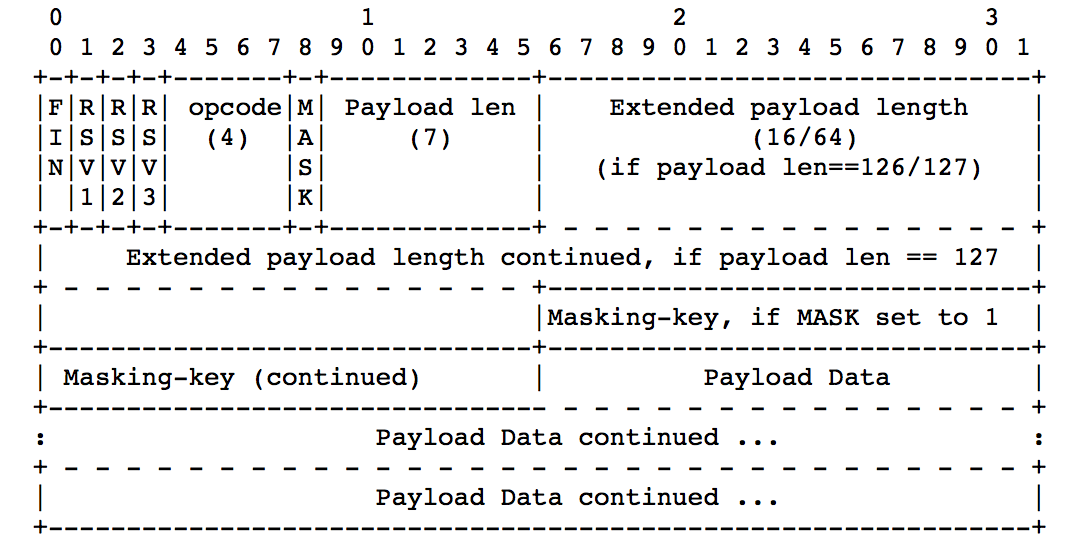
\includegraphics[width=100mm]{wire_format.png}
    \caption{wire-format di un pacchetto WebSocket}
    \label{fig:wireformat}
\end{figure}
\\Usando come riferimento l' \href{https://tools.ietf.org/html/rfc6455#section-5.2}{RFC6455}, riportiamo i significati dei vari campi:
% Campi del pacchetto
\begin{itemize}
  \item \textbf{FIN}\\
  Tale campo, di dimensione 1 bit, indica se il pacchetto corrente, rappresenta il frammento finale. È importante notare che il primo frammento \textbf{potrebbe} anche essere l'ultimo.
  \item \textbf{RSV1, RSV2, RSV3}\\
  Tali campi, ognuno di dimensione 1 bit, devono essere posti a 0, fatta eccezione per i casi in cui si sia negoziato un differente significato per tali valori.
  Possiamo considerare questi campi come riservati e quindi, a meno di opportuni accordi tra il server e il client, essi dovranno essere posti a 0, pena la chiusura della connessione.
  
  \item \textbf{Opcode}\\
  Definisce il \textit{tipo} del payload trasportato secondo la lista seguente:
  \begin{itemize}
      \item \textbf{0}: indica un frame di \textit{continuazione}
      \item \textbf{1}: indica un frame che trasporta un messaggio di testo (con codifica \textit{UTF-8}\footnote{Più informazioni su UTF-8 possono essere trovate sul sito del IETF: \href{https://tools.ietf.org/html/rfc3629}{https://tools.ietf.org/html/rfc3629}})
      \item \textbf{2}: indica un frame con un payload di dati binari
      \item \textbf{3-7}: è un range riservato per futuri frame non di controllo
      \item \textbf{8}: indica un frame di \textit{Connection Close} 
      \item \textbf{9}: indica un frame di tipo \textit{Ping}
      \item \textbf{A}: indica un frame di tipo \textit{Pong}
      \item \textbf{B-F}: è un range riservato per futuri frame di controllo
  \end{itemize}
  \item \textbf{Mask}\\
  Definisce se il campo \textit{Payload data} è \textit{mascherato}.
  Se è impostato a 1, deve essere presente il campo \textit{masking-key} che sarà utilizzato per decodificare il payload.
  Tutti i pacchetti inviati dal client verso il server dovranno avere questo bit impostato a 1.
  \item \textbf{Payload Length}\\
  Questo campo indica la lunghezza del payload in byte se il suo valore è compreso nell'intervallo [0-125].\\Se il campo assume valore 126, i successivi 2 bytes dell'intestazione andranno interpretati come un valore di intero a 16 bit (unsigned) che rappresenta la lunghezza del payload.\\
  Se il campo ha valore 127, i successivi 8 bytes dovranno essere interpretati come un intero (unsigned) di 64 bit.
  \item \textbf{Masking-key}\\
  Nel caso in cui il campo \textit{mask} fosse impostato a 1 sarà presente la chiave di 32 bit (4 byte), altrimenti sarà vuoto.
  \item \textbf{Payload data}\\
  Tale campo è costituito da due parti:
  \begin{itemize}
    \item \textbf{Extension data}\\
    Questo campo è di 0 byte a meno che non sia stata negoziato diversamente. Se presente, la sua lunghezza deve essere compresa nella lunghezza totale del payload.
    \item \textbf{Application data}\\
    La lunghezza del campo è definita come la lunghezza del payload totale meno la lunghezza dell'\textit{Extension Data}
  \end{itemize}
\end{itemize}


\section{Frame di controllo}
I frame di controllo sono identificati dal campo \textit{Opcode}.
I valori di opcode per i frame di controllo sono: 0x8 (Close), 0x9 (Ping), e 0xA (Pong), mentre i valori compresi nell'intervallo 0xB-0xF sono riservati per futuri frame di controllo ancora da definire.
Secondo lo standard tutti i frame di controllo devono avere una \textit{payload length} minore o uguale a 125 bytes e \textbf{non può} essere frammentato.
Analizziamo più nel dettaglio i vari frame di controlli.
\begin{itemize}
    \item \textbf{Close}\\
    Un frame Close è caratterizzato da un opcode con valore 0x8.
    Solitamente, è considerata buona norma indicare il motivo della chiusura della connessione all'interno dell'\textit{Application data}.
    Quando viene ricevuto un frame Close, se non ne è già stato ricevuto uno in precedenza, è necessario rispondere con un frame Close.
    Dopo aver inviato e ricevuto un messaggio di tipo Close, sia la connessione WebSocket sia quella TCP, devono essere immediatamente chiuse.

\item \textbf{Ping}\\
    Un frame di tipo Ping ha valore opcode 0x9.
    Alla ricezione di un ping il server dovrebbe rispondere con un Pong a meno che non sia stato già ricevuto un frame Close.
    Solitamente un Ping viene inviato subito dopo lo stabilimento della connessione e poco prima della chiusura per sapere se la connessione è attiva.
    Infatti i Ping vengono utilizzati anche per tenere attiva la connessione (\textit{keep-alive}).
\item \textbf{Pong}\\
    Un frame Pong deve avere un opcode con valore 0xA e deve contenere gli stessi \textit{Application data} del Ping a cui risponde.
\end{itemize}
\part{Conclusioni}
\chapter{Possibili problemi delle WebSocket}
Ogni nuova tecnologia porta con sè dei problemi, eventualmente destinati a diminuire con il passare del tempo e con la diffusione del protocollo.\\
Analizziamo quali siano i vincoli che WebSocket porta con sè.
\section{Ottimizzazione}
Il protocollo, se pur innovativo e con delle ottime prestazioni, non ha ancora raggiunto i livelli di ottimizzazione di HTTP (\textit{Caching}, \textit{Proxy}).
Del resto HTTP è utilizzato come protocollo web di tipo \textit{general-purpose}.
Infatti l'uso di vecchie tecnologie rimane ancora il più utilizzato, tanto che la maggior parte degli applicativi fa ancora uso di vecchie tecnologie come il \textit{long-polling} per ottenere servizi di aggiornamento in tempo reale.\\
\section{Diffusione}
Il protocollo WebSocket invece risulta ancora poco diffuso.
Inoltre se pur esistono diverse librerie che fanno uso di WebSocket, come ad esempio \textit{socket.io}, la documentazione sulle WebSocket è abbastanza scarsa da scoraggiare eventuali sviluppatori.
\section{Proxy}
Il protocollo WebSockets nasce con l'idea di rimanere il più possibile invisibile ai proxy.
Tuttavia l'utilizzo del metodo \textit{Upgrade} di HTTP per il cambio di protocollo rappresenta un ostacolo.
Molti proxy non permettono l'instaurazione della connessione tramite Upgrade e troncano la connessione, rendendo impossibile il completamento dell'hanshake.\\
Per fare ciò, del resto, è sufficiente che il proxy analizzi l'header HTTP e che filtri l'header \textit{Upgrade}.
\chapter{Quando usare le WebSocket}
Le possibili applicazioni di WebSocket, come già visto, sono particolarmente convenienti soprattutto per applicativi che necessitano di connessioni \textit{realtime}, con bassa \textit{latency} e bidirezionali.
Inoltre, grazie all'utilizzo della porta 80 e il sistema di upgrade della connessione, il protocollo non trova difficoltà nell'attraversamento di \textit{firewall}.\\
Alcune delle sue possibili applicazioni sono:
\begin{itemize}
    \item \textbf{Giochi multiplayer online}\\
    La bassa \textit{latency} e la comunicazione \textit{full-duplex} fornita dal protocollo candidano WebSocket come protocollo ideale per applicativi come giochi online.
    \item \textbf{Chat e altre applicazioni di comunicazione in tempo reale}\\
    WebSocket adempie al suo compito offrendo delle ottime prestazioni \textit{server-side}.
    Infatti considerando uno scenario in cui un server debba servire numerosi utenti, WebSocket offre prestazioni notevolmente superiori rispetto ai metodi tradizionali.
    \item \textbf{Applicazioni che necessitano aggiornamento in tempo reale}
    Fanno parte di questa categoria le applicazioni che necessitano un aggiornamento in tempo reale come applicazioni di transizioni monetarie o sistemi di notifiche sportive.
    \item \textbf{Applicazioni multi-utente in tempo reale}\\
    Le applicazioni multiutente di scrittura in tempo reale, come \textit{Google Docs}, rientrano in questa categoria, dove la comunicazione \textit{full-duplex} rappresenta un notevole vantaggio.
\end{itemize}
\chapter{Consigli pratici per l'uso delle WebSocket}
\section{Mitigazione di attacchi DoS (\textit{Layer7})}
Si potrebbe verificare uno scenario in cui un attaccante voglia esaurire la memoria del server inviando grossi frame dell'ordine di $2^{64}$ bytes, o più frame di dimensione totale, ovvero la dimensione del pacchetto riassemblato, ancora maggiore.\\
Una soluzione potrebbe essere quella di imporre un limite massimo sulla dimensione sia del singolo frame che della dimensione totale del pacchetto riassemblato.
\section{Compatibilità}
Ormai tutti i maggiori browser hanno aggiunto il supporto a WebSocket,
tuttavia, nella progettazione di un'applicazione capita spesso di dover rendere l'applicativo compatibile con il maggior numero possibile di dispositivi, anche quelli più datati.
A tale scopo è consigliato garantire una procedura di retrocompatibilità (\textit{fallback}) con tecnologie maggiormente supportate come il long-polling.
\section{Sicurezza}
Il protocollo WebSocket pur venendo incontro a numerose esigenze, non risolve i problemi legati sicurezza.
Un primo suggerimento è quello di progettare cautamente l'handshake HTTP agendo sulla risposta HTTP nel campo \textit{Access-Control-Allow-Origin} in modo tale da stabilire la connessione solo con origini desiderate (\textit{origin-based security policy}).
È consigliata anche l'applicazione di buone norme di sicurezza quali l'utilizzo di sistemi di autenticazione tramite sessioni/cookie o la validazione dell'input da parte del server e la corretta gestione di eventuali errori.

%\part{}
%\chapter{ Chapter}
%\lipsum[1]
    
\end{document}